\documentclass{standalone}

\usepackage{tikz}

\tikzset{wop/.style = {blue, very thick},
  rop/.style = {brown, very thick}}

% interval for operations
\newcommand{\itv}[5]{ % #1: start point; #2: end point; #3: operation name; #4: style; #name
  \coordinate (start #3) at #1;	% start point
  \coordinate (end #3) at #2;	% end point

  \draw[#4, |-|] (start #3) -- (end #3) % draw the interval
  node[pos = 0.5, above = 1mm, font = \Large] (#5) {\textsl{#3}}; % attach the operation name
}

\begin{document}
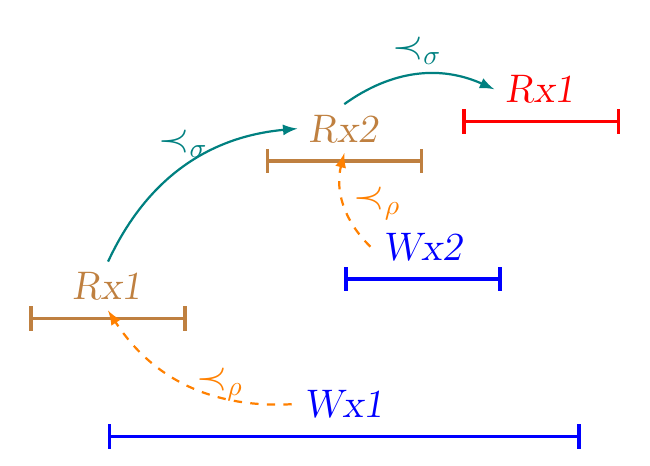
\begin{tikzpicture}
  \itv{(1,0)}{(7,0)}{Wx1}{wop}{wx1}
  \itv{(0,1.5)}{(2,1.5)}{Rx1}{rop}{rx1}
  \itv{(4,2)}{(6,2)}{Wx2}{wop}{wx2}
  \itv{(3,3.5)}{(5,3.5)}{Rx2}{rop}{rx2}

  \itv{(5.5,4)}{(7.5,4)}{Rx1}{rop, red}{rx1'}

  % wx1 -> rx1
  \draw[>=latex, ->, dashed, thick, orange, bend left] 
	(wx1.west) to node [right, font = \Large] {$\prec_{\rho}$} (rx1.south);
  % wx2 -> rx2
  \draw[>=latex, ->, dashed, thick, orange, bend left] 
	(wx2.west) to node [right, font = \Large] {$\prec_{\rho}$} (rx2.south); 
  % rx1 -> rx2
  \draw[>=latex, ->, thick, teal, bend left]
	(rx1.north) to node [above, font = \Large] {$\prec_{\sigma}$} (rx2.west);
  % rx2 -> rx1'
  \draw[>=latex, ->, thick, teal, bend left]
	(rx2.north) to node [above, font = \Large] {$\prec_{\sigma}$} (rx1'.west);
\end{tikzpicture}
\end{document}
